\documentclass[12pt,a4paper,openright]{mwrep}

\usepackage{lmodern}
\usepackage[T1]{polski}
\usepackage[utf8]{inputenc}

\usepackage[a4paper,
            tmargin=2cm,
            bmargin=2cm,
            lmargin=2cm,
            rmargin=2cm,
            bindingoffset=0cm]{geometry}

\usepackage{tocloft}
\usepackage{hyperref}

\usepackage{amsmath}
\usepackage{amssymb}
\usepackage{siunitx}

\usepackage{listings}

\usepackage{graphicx}
\usepackage{subfig}
\usepackage{float}

\hypersetup{
    colorlinks,
    citecolor=black,
    filecolor=black,
    linkcolor=black,
    urlcolor=black
}

\newtheorem{definition}{Def}

\begin{document}

\title{%
Technika cyfrowa\\
Sprawozdanie 2\\
}

\author{\\Jan Chyczyński\\Błażej Nowicki
\\Bartłomiej Słupik\\Przemysław Węglik}

\date{\today}

\maketitle

\chapter{Zadanie 2a}

\section{Wstęp}
Zadanie polega na zaprojektowaniu układu realizującego przerzutnika RS w oparciu o bramki NAND.

\begin{figure}[H]
    \centering
    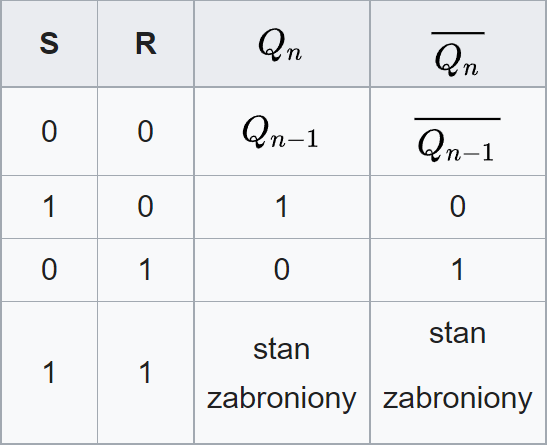
\includegraphics[width=0.5\textwidth]{images/RS_table.png}
    \caption{Tabela stanów}
    \label{rys:RS_table}
\end{figure}

\begin{figure}[H]
    \centering
    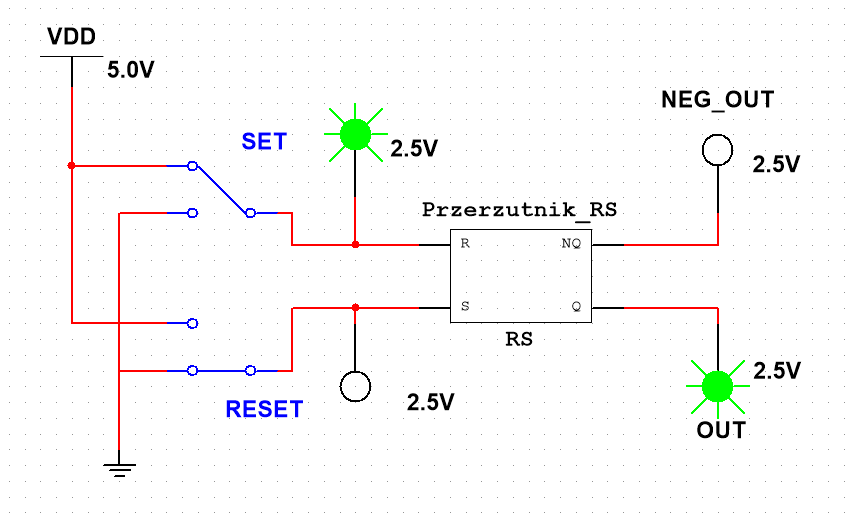
\includegraphics[width=0.8\textwidth]{images/2a_circuit_blackbox.png}
    \caption{Schemat idei rozwiązania}
    \label{rys:2a_circuit_blackbox}
\end{figure}



\section{Rozwiązanie teoretyczne}
Pierwszym krokiem jest przekształcenie wyrażenie do zawierającego
wyłączenie operacje NAND.
\begin{align*}
    Y &= \overline{A}C + B(A + B) \\
    &= \overline{\overline{\overline{A}C}\overline{B}}
\end{align*}

\section{Symulacja w programie Multisim}
Program został napisany w~języku~Python w wersji 3.8.
Do stworzenia aplikacji graficznej użyto
biblioteki~pygame\footnote{\url{https://www.pygame.org}}.

\section{Wnioski}
\begin{enumerate}
    \item Dzięki prawom logiki możemy uprosić skomplikowane wyrażenia
    w taki sposób, aby używały mniejszej ilości operacji logicznych.
    \item Przedstawienie funkcji logicznej tylko za pomocą bramek NAND
    ma praktyczne zastosowanie, ponieważ komeryjnie dostępne chipy często
    zawierają kilka bramek tego samego rodzaju (np. 4xNAND, 4xOR itp.).
    Dzięki uproszczeniu układu do bramek NAND, możemy go skonstruować
    w rzeczywistościu używając tylko jednego chipu 4xNAND zamiast
    trzech różnych: 4xNOT, 4xOR i 4xAND.
    \item Podana funkcja logiczna po drobnym przekształceniu
    \begin{align*}
        Y = \overline{A}C + B(A + B) = \overline{A}C + B
    \end{align*}
    przedstawia równanie charakterystyczne przerzutnika 
    asynchronicznego typu RS. 
    Po podstawieniach
    \begin{align*}
        A &= R\\
        B &= S\\
        C &= Q_{n-1}\\
        Y &= Q_{n}\\
    \end{align*}
        
    otrzymujemy
    \begin{align*}
        Q_{n} = S + \overline{R}Q_{n-1}
    \end{align*}


\end{enumerate}


\end{document}
